%%%%%%%%%%%%%%%%%%%%%%%%%%%%%%%%%%%%%%%%%
%
% CMPT 435
% Lab Zero
%
%%%%%%%%%%%%%%%%%%%%%%%%%%%%%%%%%%%%%%%%%

%%%%%%%%%%%%%%%%%%%%%%%%%%%%%%%%%%%%%%%%%
% Short Sectioned Assignment
% LaTeX Template
% Version 1.0 (5/5/12)
%
% This template has been downloaded from: http://www.LaTeXTemplates.com
% Original author: % Frits Wenneker (http://www.howtotex.com)
% License: CC BY-NC-SA 3.0 (http://creativecommons.org/licenses/by-nc-sa/3.0/)
% Modified by Alan G. Labouseur  - alan@labouseur.com, and Patrick Tyler - Patrick.Tyler1@marist.edu
%
%%%%%%%%%%%%%%%%%%%%%%%%%%%%%%%%%%%%%%%%%

%----------------------------------------------------------------------------------------
%	PACKAGES AND OTHER DOCUMENT CONFIGURATIONS
%----------------------------------------------------------------------------------------

\documentclass[letterpaper, 10pt]{article} 

\usepackage[english]{babel} % English language/hyphenation
\usepackage{graphicx}
\usepackage[lined,linesnumbered,commentsnumbered]{algorithm2e}
\usepackage{listings}
\usepackage{fancyhdr} % Custom headers and footers
\pagestyle{fancyplain} % Makes all pages in the document conform to the custom headers and footers
\usepackage{lastpage}
\usepackage{xcolor}
\usepackage{url}
\usepackage{titlesec}

% Stolen from https://www.overleaf.com/learn/latex/Code_listing 
\definecolor{codegreen}{rgb}{0,0.6,0}
\definecolor{codegray}{rgb}{0.5,0.5,0.5}
\definecolor{codepurple}{rgb}{0.58,0,0.82}
\definecolor{backcolour}{rgb}{0.95,0.95,0.92}

\lstdefinestyle{mystyle}{
    backgroundcolor=\color{backcolour},   
    commentstyle=\color{codegreen},
    keywordstyle=\color{magenta},
    numberstyle=\tiny\color{codegray},
    stringstyle=\color{codepurple},
    basicstyle=\ttfamily\footnotesize,
    breakatwhitespace=false,         
    breaklines=true,                 
    captionpos=b,                    
    keepspaces=true,                 
    numbers=left,                    
    numbersep=5pt,                  
    showspaces=false,                
    showstringspaces=false,
    showtabs=false,                  
    tabsize=2
}
\lstset{style=mystyle, language=c++}


\fancyhead{} % No page header - if you want one, create it in the same way as the footers below
\fancyfoot[L]{} % Empty left footer
\fancyfoot[C]{page \thepage\ of \pageref{LastPage}} % Page numbering for center footer
\fancyfoot[R]{}

\renewcommand{\headrulewidth}{0pt} % Remove header underlines
\renewcommand{\footrulewidth}{0pt} % Remove footer underlines
\setlength{\headheight}{13.6pt} % Customize the height of the header

%----------------------------------------------------------------------------------------
%	TITLE SECTION
%----------------------------------------------------------------------------------------

\newcommand{\horrule}[1]{\rule{\linewidth}{#1}} % Create horizontal rule command with 1 argument of height

\title{	
   \normalfont \normalsize 
   \textsc{CMPT 435 - Fall 2023 - Dr. Labouseur} \\[10pt] % Header stuff.
   \horrule{0.5pt} \\[0.25cm] 	% Top horizontal rule
   \huge Assignment Four -- \LaTeX ~DP and Greedy\\     	    % Assignment title
   \horrule{0.5pt} \\[0.25cm] 	% Bottom horizontal rule
}

\author{Patrick Tyler \\ \normalsize Patrick.Tyler1@marist.edu}

\date{\normalsize\today} 	% Today's date.

\begin{document}
\maketitle % Print the title
\section{Dynamic Programming}
Dynamic programming (DP) is the computer science technique of using results from a previous calculation
is the rest of the program (breaking problems into smaller pieces). This is especially useful when you have expensive pure functions 
(a function which returns the same value for the same input and has no side effects).
A popular problem which benefits heavily from a DP approach is calculating
the fibonacci sequence recursively. There is a lot of identical calls when calculating the fibonacci sequence.
So, if the results are cached a lot of computation can be saved as demonstrated in figure \ref{fig:fib}.
\begin{figure}[h]
    \centering
    % source: https://avikdas.com/2019/04/15/a-graphical-introduction-to-dynamic-programming.html
    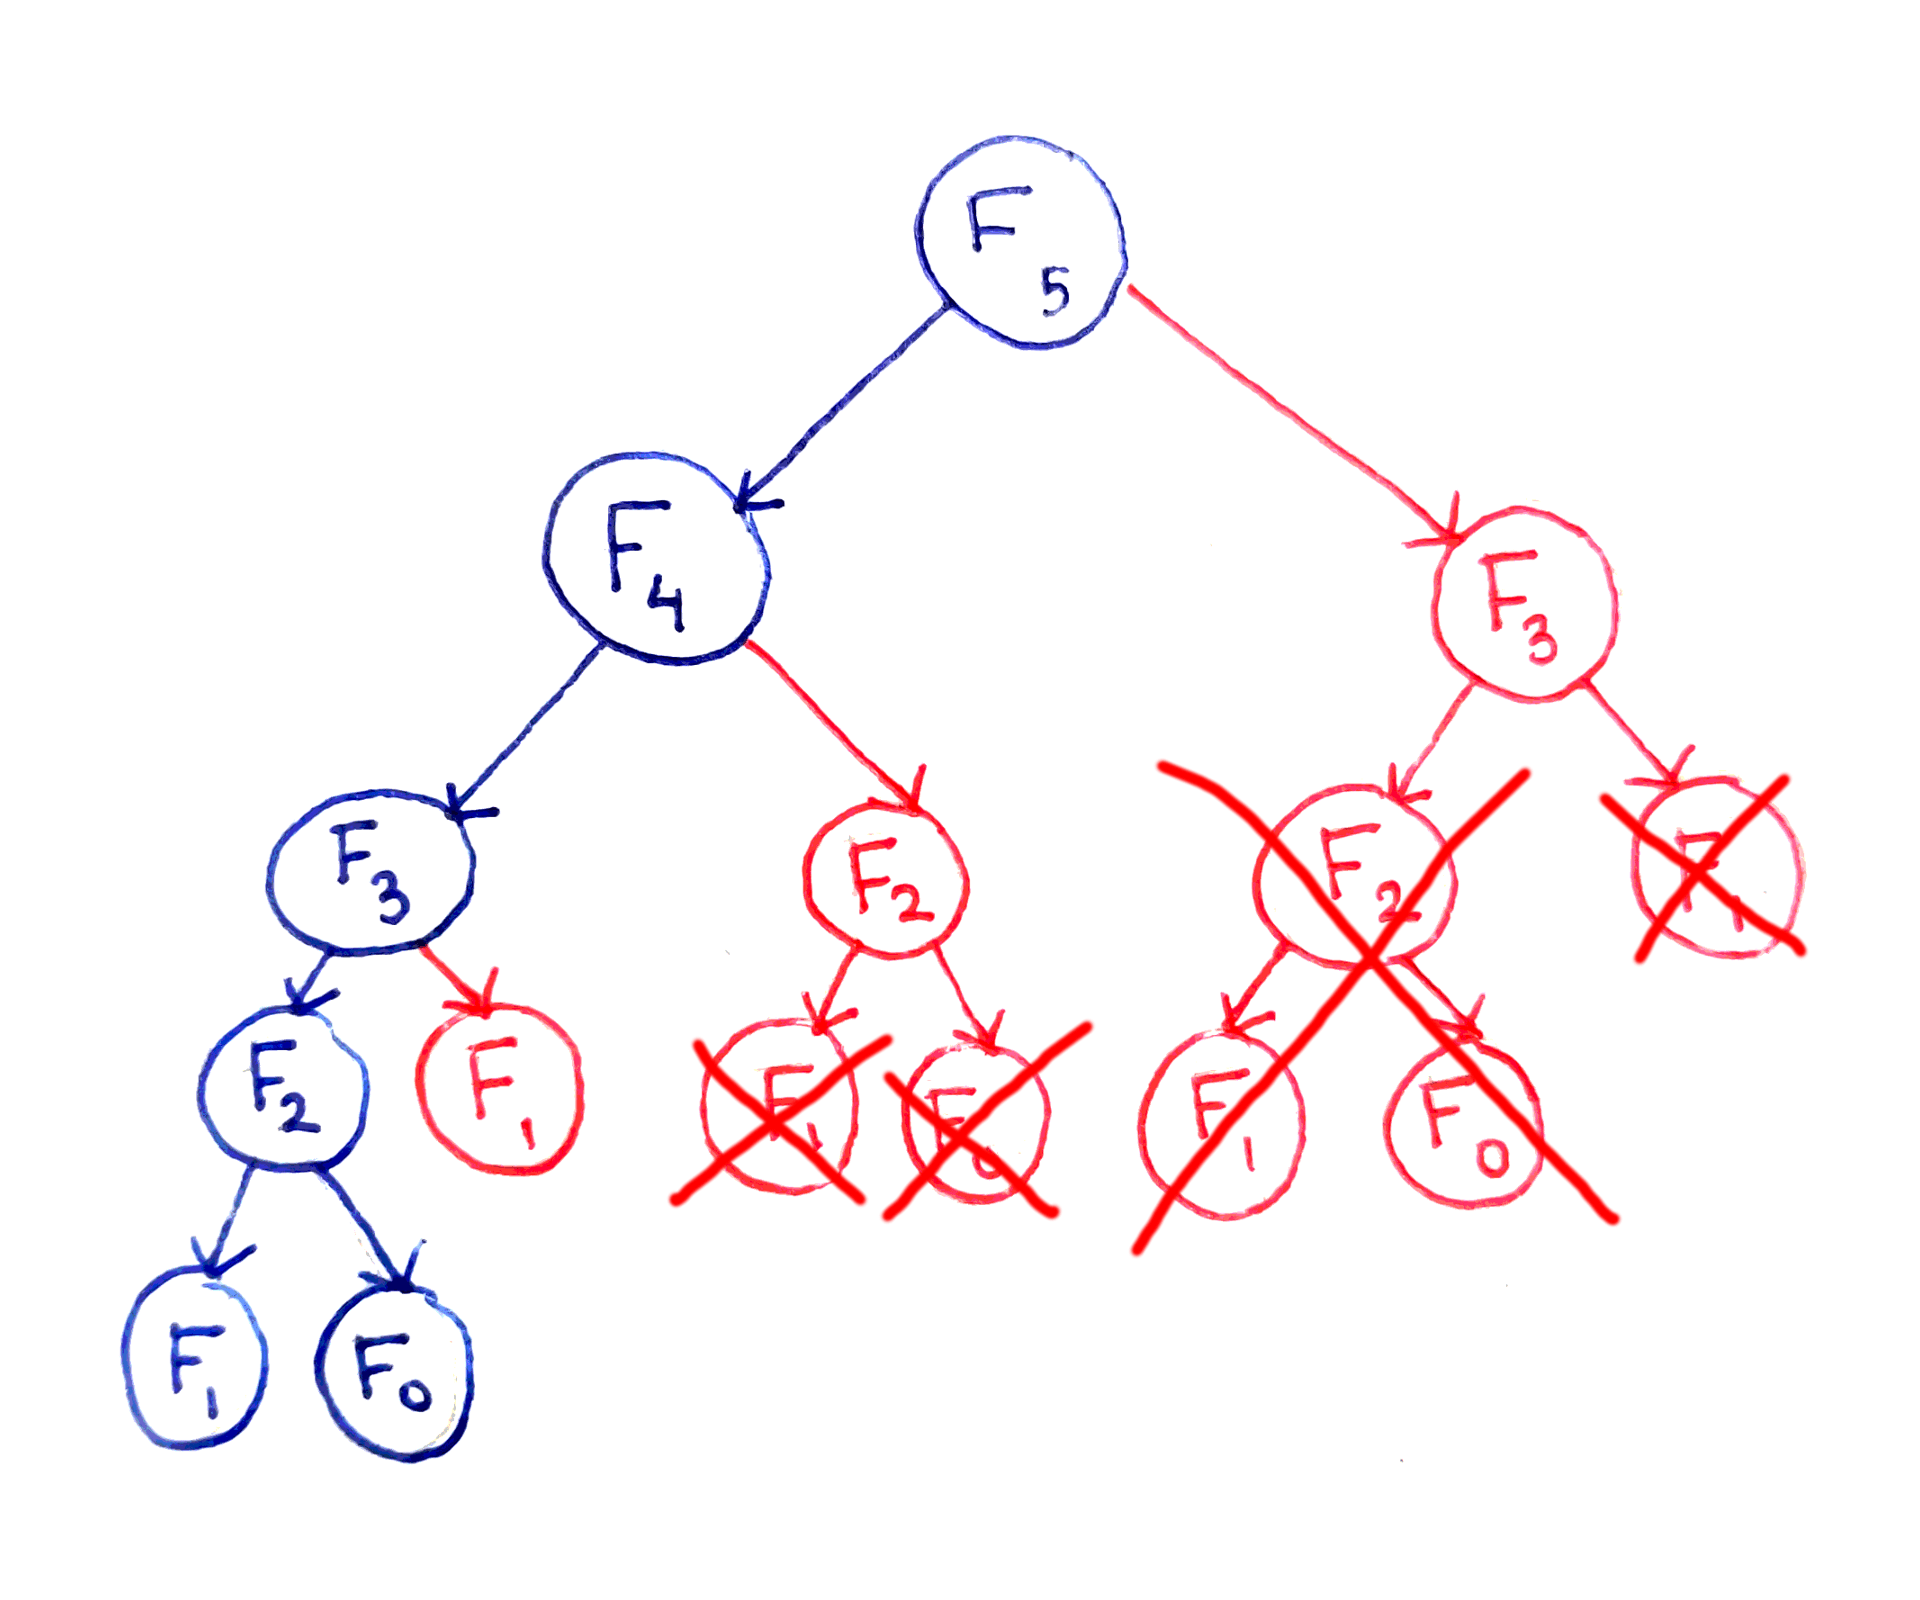
\includegraphics[width=.55\textwidth]{fibonacci-memoized.png}
    \caption{Fibonacci Sequence from Avik Das}
    \label{fig:fib}
\end{figure}
\newpage
\subsection{Bellman Ford Algorithm}
Another algorithm which takes advantage of DP is the Bellman Ford algorithm. This algorithm finds the shortest distances
from a source vertex to the other reachable vertices in a weighted graph. The steps of this algorithm are as follows:\\
\begin{enumerate}
  \item Initialize storage of current distance values and predecessors. The starting distance from the starting vertex should always compare as greater than a finite distance so infinity is used. The distance from the starting vertex to itself is 0.
  
  \lstinputlisting[linerange={244-249}, firstnumber=244]{main.cpp}
  
  \item For each edge check where $u$ is the \textbf{from} vertex, $v$ is the \textbf{to}, and its distance is defined as the stored shortest path from the starting point. Check if $u$'s distance plus the edge weight is less than $v$'s current weight. If that check is true, then update the distance with the shortest value and $v$'s predecessor to $u$. The checking and updating process is generally referred to as "relaxing" the edge.
  
  \lstinputlisting[linerange={254-268}, firstnumber=254]{main.cpp}
  
  \item Repeat step 2 until it has been completed one less than the count of vertices. This ensures that the algorithm has enough iterations to propagate the distance values at most the count of vertices minus 1 out. This should be intuitive because any given vertex can be at most vertices count minus 1 edges away from the starting vertex if it is reachable at all.
  
  \item Check for any negative edge cycles. If one of these exists, then the minimum path is indefinitely small/negative infinity. This step is essentially the same as 2, but if there is any spot where the condition is true then there are negative cycle(s).
  
  \lstinputlisting[linerange={272-287}, firstnumber=272]{main.cpp}
\end{enumerate}
The following time complexities are based off these variables: \(|V|\) is the number/ cardinality of vertices and \(|E|\)
is the number/ cardinality of edges. It is worth noting that \(0 <= |E| <= |V|^2\) so substitutions can be made.
\begin{enumerate}
    \item Time complexity \(O(|V|)\) because it does some work for each vertex.
    \item Time complexity \(O(|E|)\) because it does some work for each edge.
    \item Time complexity \(O(|V|*|E|)\) because it does step 2 for each vertex.
    \item Time complexity \(O(|E|)\) because it does some work for each edge.
\end{enumerate}
Overall this algorithm takes on the time complexity \(O(|V|*|E|)\). It is important to note that due to this implementation
of edge storage step 2 must at least loop through all vertices even if there is no edge on those vertices.
\vspace{.25cm}
\hrule
\vspace{.25cm}
\noindent
% Sorry for the bad jokes it's hard for this section
Student: \textit{Hey Professor, why did I get a 0 on my DP homework?}\\
Professor: \textit{It was copied. I literally found the exact code online.}\\
Student: \textit{Yup, why do the work when we can already lookup the answer that's DP 101 right?}\\
Professor: \textit{You're a moron.}\\
\hrule
\vspace{1cm}

\newpage
\section{Greedy Algorithms}
A greedy algorithm takes locally optimal solutions to approximate a globally optimal solution.
Giving optimal change is a great example of how a problem can benefit from a greedy approach even
if it needs a DP backtracking approach in certain cases. With US currencies you can always
find the optimal change (least amount of bills and or coins) with the diagramed greedy method: taking the highest denomination
that fits adding that to change and repeating the process with what is leftover as seen in figure \ref{fig:greedy}.
If the problem had any set of valid denominations this would not be possible with a greedy approach.
For instance, if you had this set of currencies \{20, 9, 1\} and need to give 28 dollars of change, the solution
from the greedy approach would be \{20, 1 x 7\}. However, the optimal solution is \{9 x 3, 1\}.
% MISTUNDERTAND DP USING PLAGAREIS
% Following example from https://en.wikipedia.org/wiki/Greedy_algorithm
\begin{figure}[h]
    \centering
    % source: https://en.wikipedia.org/wiki/Greedy_algorithm#/media/File:Greedy_algorithm_36_cents.svg
    \includegraphics[width=.5\textwidth]{greedy.png}
    \caption{Change diagram and example from wikipedia}
    \label{fig:greedy}
\end{figure}
\subsection{Spice Heist}
The intergalactic Spice Heist is a flavor of the knapsack problem. Which much like the currency 
problem has a subproblem, all or none nothing knapsack, where a greedy solution does not produce 
a globally optimal answer. In this heist, however, it is permissable to take any fraction
of spices. This version allows for a the greedy approach much like giving change with denomination that
are multiples of each other: simply just take all of the most cost-effective spices first until the sack
is at capacity or there are no more spices to take. \\
\newline
The time complexity depends on the sorting implemented.
The implementation in the index uses a binary search tree (without balancing) to sort the spices. As each spice
is inserted it takes \(O(n)\) to correctly insert it in the BST (think of the stick BST from previous the assignment) 
for its given where n is the amount of spices
currently in the BST. However, it will likely only take a little over \(log_2n\) operations if the spices are randomly
arranged in terms of the unit cost. This operation happens \(n\) times so therefore adding all spices is a \(O(n^2)\)
operation, but more likely around \(nlog_2n\) operations will be done. Getting the spices sorted from the tree is
done through an in-order traversal and the elements are appended to a vector for convenience. Retrieving this vector
in the doHeist function takes \(O(n)\) time if the vector has not been retrieved since last insertion or is constant time if
the sorted vector is already stored. Then, looping through the spices to and doing checks to add the most amount is \(O(n)\).
This makes the overall process of adding spices and generating the best knapsack for a given capacity \(O(n^2)\).
  \lstinputlisting[linerange={563-588}, firstnumber=563]{main.cpp}
\vspace{.25cm}
\hrule
\vspace{.25cm}
\noindent
% Sorry for the bad jokes it's hard for this section
\textbf{Guy:}\\
Why do we call politicians greedy? \textit{Because they make locally optimal solutions to extend their power with the global consequences of screwing future generations.}\\
\textbf{Interviewer:}\\
Sir, the question was: \textit{What is a greedy algorithm?}
\hrule
\newpage
\section{Miscellaneous}
As always the source code can be found in the index. The chosen way to do the file
reading and parsing was incredibly stupid and probably not even more efficient than
easier and more readable approaches. You can look at the commit messages to 
get a better understanding of my frustrations. However, the parsing should not take
all the credit for my frustrations, because I thought the raw binary output (mounds of red text)
was from incorrect parsing when it was really from bad memory management.\\
\newline
Here's a C++ exercise for the reader. Which copy has a likely bug in it? \\
Source code and latex has the answer but the explanation can be found below.
\begin{lstlisting}[]
        // other function stuff
        Spice* spice = new Spice();
        spice->name = name;
        spice->price = totalPrice;
        spice->quantity = quantity;
        spice->unitCost = totalPrice / quantity;
        this->spices->insert(spice);
        // end of function
\end{lstlisting}

% This listing below is the problem
\begin{lstlisting}[]
        // other function stuff
        Spice spice = (*new Spice()); 
        spice.name = name;
        spice.price = totalPrice;
        spice.quantity = quantity;
        spice.unitCost = totalPrice / quantity;
        this->spices.insert(&spice);
        // end of function
\end{lstlisting}
The problem is that C++ automatically garbage collects the Spice object that is
dereferenced in the function and therefore my BST was storing pointers to collected objects. 
When I was debugging this I printed the attributes as they were being adding which obviously still worked
and left me very confused, because the only problem was mounds of raw binary bad encoding being output
when I was printing it later.
\end{document}
